\scanpage{10}
\uline{Corollaire} Soit $u:H-G$ un hom de préschémas en groupes \inserted{sur $S$}, avec $G$ loc. noeth., \inserted{et \deleted{séparé sur $S$}}, $H$ de type fini sur $S$, \deleted{Alors} $H$ \inserted{plat et} satisfaisant la condition $R$ (p.ex. : fibres connexes\ldots). \inserted{\deleted{Si $G$ séparé sur $S$}} Alors $\uline{\operatorname{Cent}}_G(u)$ est représentable par un sous-préschéma \deleted{fermé} de $G$, \deleted{Corollaire} fermé si $G$ est séparé sur $S$.

Si $K$ est un sous-groupe de $G$, \deleted{Alors} \deleted{de \unsure{t.f.}} \inserted{de t.f. sur $\unsure{K|S}$} $\uline{\operatorname{Transp}}_G(u,K)$ est représentable, et si $K$ est un sous-préschéma de $G$ (resp. sous-préschéma fermé de $G$) il en est de $=$ de $\uline{\operatorname{Transp}}_G(u,K)$. Enfin, si \deleted{un $H$} $K$ est également plat \deleted{et} sur $S$ et satisfait la condition $R$, \deleted{alors $\operatorname{Transp}_G$} et $u$ une \uline{imm}, alors \deleted{$\operatorname{Transp}_G(u,K)$} $\operatorname{Transp}.^{\unsure{*|\simeq}}_G(H,K)$ est représentable par un \deleted{\unsure{sous-groupe}} schéma de type fini sur $G$, et c'est un sous-préschéma (resp. sous-préschéma fermé) s'il en est de $=$ de $H$ et $K$ dans $G$.

En particulier, $\uline{\operatorname{Norm}}_G(H)$ est représentable, c'est un sous-préschéma (resp. sous-préschéma fermé) \inserted{de $G$} si $H$ l'est.
\figure{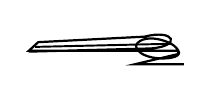
\begin{tikzpicture}[x=1cm,y=1cm]\draw[line width=.8pt] (0,0)--(1.55,.04) .. controls (1.95,.07) and (1.85,.29) .. (1.47,.19)--(.12,.12)--(0,.01)--(1.9,.01) .. controls (1.99,-.12) and (1.38,-.14) .. (1.36,.08) .. controls (1.46,.27) and (1.94,.11) .. (1.9,-.03)--(1.35,-.16)--(1.97,-.16);\draw[line width=.7pt] (.08,.06)--(1.82,.1);\end{tikzpicture}}
\mspage{9}
